\documentclass[letterpaper]{article}
\usepackage{proceed2e}
\usepackage[margin=1in]{geometry}
\usepackage{mathtools}
\usepackage{amsfonts}
\usepackage{amsthm}
\usepackage{subfig}
\usepackage{hyperref}

\usepackage{times}
\usepackage{float}

\usepackage{natbib}

\newtheorem{theorem}{Theorem}
\newtheorem{lemma}{Lemma}

\allowdisplaybreaks

\title{Uncertainty propagation in deep neural networks for sparse coding}

\author{} % LEAVE BLANK FOR ORIGINAL SUBMISSION.
          % UAI  reviewing is double-blind.

% The author names and affiliations should appear only in the accepted paper.
%
%\author{ {\bf Harry Q.~Bovik\thanks{Footnote for author to give an
%alternate address.}} \\
%Computer Science Dept. \\
%Cranberry University\\
%Pittsburgh, PA 15213 \\
%\And
%{\bf Coauthor}  \\
%Affiliation          \\
%Address \\
%\And
%{\bf Coauthor}   \\
%Affiliation \\
%Address    \\
%(if needed)\\
%}

\author{ {\bf Danil Kuzin} \\
\And
{\bf Olga Isupova}  \\
\And
{\bf Lyudmila Mihaylova}   \\
}

\begin{document}

\maketitle

\begin{abstract}
We propose the method of propagating the uncertainty through the multilevel soft-thresholding nonlinearity. This allows to use it as a building block for sparse coding deep neural networks. As an example we develop the Bayesian LISTA algorithm with probabilistic backpropagation. It allows to obtain the variance estimates for parameters and posterior distributions.
\end{abstract}

\section{Introduction}
Though the idea of Bayesian learning in neural networks is not new \citep{neal2012bayesian}, it has gained its attention only recently, with the development of distributed approximate inference techniques \citep{li2015stochastic, hoffman2013stochastic}  and general boost in popularity of deep learning. In some spheres, such as self-driving cars or healthcare, posterior estimates are very important and Bayesian learning allows to obtain them. 

In general, when distributions are included in the network, Bayesian inference complexity scales exponentially with the number of layers, thus making it difficult to be implemented for deep neural networks in general. Nevertheless, recently several techniques were proposed to handle specific types of neural networks. For example, dense layers \citep{hernandez2015probabilistic}, networks with discrete distributions \citep{soudry2014expectation}, recurrent networks \citep{mcdermott2017bayesian}. 

There are currently two approaches for Bayesian neural networks: distributions of weights can be included in the network \citep{hernandez2015probabilistic, ranganath2015deep}, or dropout can be interpreted as an element introducing the uncertainty \citep{gal2016dropout}. In this paper we are using the first way and impose distributions on weights and parameters to obtain posterior estimates of parameters, weights and predictions with uncertainty estimated.

Sparse coding problem can be viewed as the linear regression problem with the additional assumption that some of the basis representation coefficients should be zeros. It arises in different applications, such as compressive sensing~\cite{candes2008introduction}, image and video processing~\cite{mairal2014sparse}, non-invasive brain activity areas discovery \cite{baillet1997bayesian}. 

The usual approach in neural networks for sparse coding is to use the soft thresholding nonlinearity, that shifts current estimates towards zero \citep{lecun2010mnist}. It allows to obtain predictions containing zeros. In this paper we propose the approach to propagate uncertainty through the soft-thresholding nonlinearity. At every layer the current distribution of the target vector is represented as spike-and-slab distribution \citep{mitchell1988bayesian}, and we show that it can be effectively combined with Gaussian weights for dense layers and after soft-thresholding it can be closely approximated with distribution from the same family.

The proposed method of uncertainty propagation for sparse coding allows to derive the gradients of the normalisation constant logarithm of the model likelihood which is used in probabilistic backpropagation to update weights distribution, therefore it can be applied to Bayesian neural networks for sparse coding.

The paper is organised as following: first, we describe the uncertainty propagation to obtain the spike-and-slab distribution - output from the network, then we describe how the backpropagation is organised to update distributions of weights and their priors. After that we show how the algorithm is performed on \textsc{mnist} data and demonstrate the obtained posterior estimates.

The main contributions are: 
\begin{itemize}
\item for the first time we propose uncertainty propagation through the soft-thresholding nonlinearity for Bayesian neural network
\item efficient posterior inference for weights and outputs of neural networks with the soft-thresholding nonlinearity
\item novel Bayesian neural network network for sparse coding
\end{itemize}

\section{Neural networks for sparse coding}

The problem of sparse coding is the linear regression with assumption of sparse weights
\begin{equation}
\label{eq:regression_problem}
\mathbf{y} = \mathbf{X}\boldsymbol\beta + \varepsilon
\end{equation}
where $\mathbf{y} \in \mathbb{R}^K$ is the observation, $\mathbf{X} \in \mathbb{R}^{K \times D}$ is the design matrix, $\boldsymbol\beta \in \mathbb{R}^D$ is unknown vector of weights such that $K < D$ with some of its elements $\beta_d$ equal to zero to achieve regularisation. $\varepsilon \in \mathbb{R}^K$ is the independent Gaussian noise.

One of the popular families of the sparse coding algorithms is the iterative shrinkage algorithms, and notably the Iterative Shrinkage and Thresholding Algorithm(\textsc{ista}) \citep{daubechies2004iterative}. It iteratively obtains the new approximation of the coefficients vector $\widehat{\boldsymbol\beta}_l$ as the linear transformation of the input $\mathbf{y}$ with previous approximation $\widehat{\boldsymbol\beta}_{l-1}$ and then propagates the new approximation through the soft thresholding function $h_\lambda(\cdot)$
\begin{equation}
h_\lambda(v) = \text{sgn}(v) \max(|v| - \lambda, 0)
\end{equation}
where $\lambda$ is a shrinkage parameter.
The linear transformation is
\begin{equation}
\widehat{\boldsymbol\beta}_l = \mathbf{W}\mathbf{y} + \mathbf{S}_l\widehat{\boldsymbol\beta}_{l-1}
\end{equation}
with weights $\mathbf{W} = \mathbf{X}^\top / E$, $E$ - upper bound on the largest eigenvalue of $\mathbf{X}^\top\mathbf{X}$ and $\mathbf{S} = \mathbf{I}_{D \times D} - \mathbf{W}\mathbf{X}$.

Learned \textsc{ista} (\textsc{lista}) \citep{gregor2010learning} algorithm allows to learn the values of matrices $\mathbf{W}$, $\mathbf{S}$. To achieve this, \textsc{ista} algorithm is limited with the fixed amount of iterations, $L$ and interpreted as a recurrent neural network. Overall, it has the following scheme
\begin{align}
&\mathbf{b} = \mathbf{W}\mathbf{y}\\
&\widehat{\boldsymbol\beta}_0 = h_\lambda(\mathbf{b}_0) \\
&\text{for } l=1:L\\
	&\quad \mathbf{c}_l = \mathbf{b} + \mathbf{S}\widehat{\boldsymbol\beta}_{l-1} \\
	&\quad \widehat{\boldsymbol\beta}_{l} = h_\lambda(\mathbf{c}_l) \\
& \widehat{\boldsymbol\beta} = \widehat{\boldsymbol\beta}_{L}
\end{align}

Matrices $\mathbf{W}$, $\mathbf{S}$ are the parameters that are initialised as in \textsc{ista} and then updated with the backpropagation algorithm. Vectors $\mathbf{c}_l$, $\mathbf{b}$ are intermediate vectors that describe forward propagation. $\boldsymbol\beta_l$ is the current approximation of the target coefficients vector.

\section{Bayesian neural network for sparse coding}
To formulate the Bayesian version of \textsc{lista} we impose the prior distributions on the unknown weights
\begin{align}
&p(\mathbf{W}) = \prod_{d=1}^D\prod_{k=1}^K \mathcal{N}(w_{ij, l} | 0, \eta^{-1}), \\
&p(\mathbf{S}) = \prod_{d'=1}^D\prod_{d''=1}^D \mathcal{N}(s_{d'd'', l} | 0, \eta^{-1}),
\end{align}
where $w_{ij, l}$ is the component of the matrix $\mathbf{W}_l$, $s_{d'd'', l}$ is the component of the matrix $\mathbf{S}_l$ from the layer $l$.
Likelihood of the output $\mathbf{y}$ is defined as 
\begin{equation}
\label{eq:likelihood}
p(\mathbf{y}; \mathbf{W}, \mathbf{S}, \gamma) = \prod_{d=1}^D\mathcal{N}([\mathbf{y}]_d; [f(\mathbf{y}; \mathbf{W}, \mathbf{S})]_d, \gamma^{-1}),
\end{equation}
where $f(\mathbf{y}; \mathbf{W}, \mathbf{S})$ is the output of the \textsc{lista} neural network.
The posterior distribution is 
\begin{equation}
\label{eq:posterior}
p(\mathbf{W}, \mathbf{S}, \gamma, \eta | D) = \frac{p(\mathbf{y} | \mathbf{W},  \mathbf{S}, \gamma) p(\mathbf{W} | \eta )p(\mathbf{S} | \eta) p(\eta) p(\gamma)}{p(\mathbf{y})}
\end{equation}
The shrinkage parameter $\lambda$ is a hyperparameter of the model.

\section{Uncertainty propagation through soft thresholding}
We initialise the $\widehat{\boldsymbol\beta}_{0}$ with the spike and slab distribution with parameters $\boldsymbol\omega = \mathbf{0}$, $\mathbf{m} = \mathbf{0}$, $\mathbf{v} = \mathbf{1}$. For every layer we assume that $\widehat{\boldsymbol\beta}_{l-1}$ has the spike and slab distribution with parameters $\boldsymbol\omega$, $\mathbf{m}$, $\mathbf{v}$
\begin{equation}
[\boldsymbol\beta_{l-1}]_d \sim [\boldsymbol\omega]_d \delta_0 + (1 - [\boldsymbol\omega]_d)\mathcal{N}([\mathbf{m}]_d, [\mathbf{v}]_d)
\end{equation}

Further in this section we show that the value of the next layer $\widehat{\boldsymbol\beta}_l$ can be approximated with spike and slab distribution and therefore it maintains the same family of distributions and allows to apply the extended probabilistic backpropagation algorithm that is proposed in Section~\ref{sec:backpropagation}: lemma \ref{thm:matrix_const} describes the probabilistic variant of \textsc{lista} step $\quad \mathbf{b}_l = \mathbf{W}_l \mathbf{y}$, lemma \ref{thm:matrix_vector} and \ref{thm:sum_vectors} describe the probabilistic variant of \textsc{lista} step $ \mathbf{c}_l = \mathbf{b}_l +\mathbf{S}$ and lemma \ref{thm:soft_thresholding} describes the soft thresholding step $\widehat{\boldsymbol\beta}_{l} = h_\lambda(\mathbf{c}_l)$. Overall the probabilistic layer is described by theorem \ref{thm:prob_layer}.

\begin{lemma}[Moments of spike and slab distribution]
\label{thm:moments_spsl}
Let the random variable $\xi$ have a spike and slab distribution with probability of spike $\omega$, slab mean $m$ and slab variance $v$. Then its moments are
\begin{subequations}
\begin{align}
\mathbb{E}\xi &= (1-\omega)m \\
\operatorname{Var}\xi & = (1-\omega)(v + \omega m^2)
\end{align}
\end{subequations}
\end{lemma}

\begin{proof}
\begin{align*}
\begin{split}
\mathbb{E}\xi &= \int x (\omega \delta_0(x) + (1 - \omega)\mathcal{N}(x; m, v))dx \\
& = \omega \int x \delta_0(x)dx + (1 - \omega)\int x \mathcal{N}(x; m, v)dx \\
& = (1-\omega)m \\
\mathbb{E}\xi^2 &= \int x^2 (\omega \delta_0(x) + (1 - \omega)\mathcal{N}(x; m, v))dx \\
& = \omega \int x^2 \delta_0(x)dx + (1 - \omega)\int x^2 \mathcal{N}(x; m, v)dx \\
& = (1-\omega)(v + m^2) \\
\operatorname{Var}\xi &= \mathbb{E}\xi^2 - \left(\mathbb{E}\xi\right)^2 = (1-\omega)(v + \omega m^2)
\end{split}
\end{align*}
\end{proof}

 \begin{lemma}[Product of Gaussian matrix and constant vector]
 \label{thm:matrix_const}
 Let $\mathbf{W} \in \mathbb{R}^{D \times K}$ be a matrix of independent Gaussian-distributed random variables: $w_{dk} \sim \mathcal{N}(m^w_{dk}, v^w_{dk})$, and $\mathbf{y} \in \mathbb{R}^K$ be a constant vector. Then their product $\mathbf{W} \mathbf{y}$ is a vector $\mathbf{b} \in \mathbb{R}^{D}$ of random variables $b_d \sim \mathcal{N}(m^b_d, w^b_d)$, where 
\begin{subequations}
\begin{align}
m^b_d &= \sum_{k=1}^Ky_k m^w_{dk}, \\
w^b_d &= \sum_{k=1}^Ky_k^2v^w_{dk}.
 \end{align}
\end{subequations}
 
 \end{lemma}
 \begin{proof}
 	The statement follows from the property that the family of normal distributions is closed under linear transformations.
 \end{proof}
 
  \begin{lemma}[Product of Gaussian matrix and Gaussian vector]
  \label{thm:matrix_vector}
 Let $\mathbf{S} \in \mathbb{R}^{D \times D}$ be a matrix of independent Gaussian-distributed random variables: $s_{d'd''} \sim \mathcal{N}(m^s_{d'd''}, v^s_{d'd''})$, and $\boldsymbol\beta \in \mathbb{R}^D$ be a vector with spike-and-slab distributed variables: $\beta_d \sim \omega_d \delta_0 + (1 - \omega_d)\mathcal{N}(m_d, v_d)$. If their product is approximated as a vector $\mathbf{e} \in \mathbb{R}^{D}$ of random variables $e_d \sim \mathcal{N}(m^e_d, w^e_d)$, then 
\begin{subequations}
\begin{align}
 m^e_d &= \sum_{d'=1}^D m^s_{dd'}(1-\omega_{d'})m_{d'}, \\
 \begin{split}
 v^e_d &= \sum_{d'=1}^D [(m^s_{dd'})^2(1-\omega_{d'})^2v_{d'} \\
 & {}+ (1-\omega_{d'})^2(m_{d'})^2v^s_{dd'} + v^s_{dd'}(1-\omega_{d'})^2v_{d'}].
 \end{split}
 \end{align}
\end{subequations}
 \end{lemma}
 \begin{proof}
 	We compute the mean and variance of the product $\mathbf{S}\boldsymbol\beta$ with an assumption of independence of its components and approximate resulting distribution with Gaussian. The quality of this approximation is discussed in section \ref{sec:approx_quality}
\begin{flalign*}
	\mathbb{E}e_d &= \sum_{d'=1}^D \mathbb{E}[s_{dd'}\beta_{d'}]  = \sum_{d'=1}^D m^s_{dd'}\mathbb{E}\beta_{d'}\\
	\operatorname{Var}e_d &= \sum_{d'=1}^D \operatorname{Var}[s_{dd'}\beta_{d'}] = \sum_{d'=1}^D [(\mathbb{E}s_{dd'})^2 \operatorname{Var}\beta_{d'} \\
	&{}+ (\mathbb{E}\beta_{d'})^2 \operatorname{Var}s_{dd'} + \operatorname{Var}\beta_{d'} \operatorname{Var}s_{dd'}]
\end{flalign*}
where $\mathbb{E}\beta_{d'}$, $\operatorname{Var}\beta_{d'}$ are computed according to lemma~\ref{thm:moments_spsl}.
 \end{proof}

\begin{lemma}[Sum of Gaussian vectors]
\label{thm:sum_vectors}
If $\mathbf{b} \in \mathbb{R}^{D}$ and $\mathbf{e} \in \mathbb{R}^{D}$ are both vectors of independent Gaussian-distributed random variables: $b_{d} \sim \mathcal{N}(m^b_{d}, v^b_{d})$, $e_{d} \sim \mathcal{N}(m^e_{d}, v^e_{d})$ then their sum $\mathbf{c} = \mathbf{b} + \mathbf{e}$ is a vector of independent Gaussian-distributed random variables $c_{d} \sim \mathcal{N}(m^c_{d}, v^c_{d})$ with 
\begin{subequations}
\begin{align}
m^c_{d} &= m^b_{d} + m^e_{d}, \\
v^c_{d} &= v^b_{d} + v^e_{d}.
 \end{align}
\end{subequations}
\end{lemma}
\begin{proof}
Based on properties of Gaussian distributions.
\end{proof}

\begin{lemma}[Gaussian propagation through soft thresholding]
\label{thm:soft_thresholding}
When a Gaussian-distributed random variable $x \sim \mathcal{N}(x; m, v)$ is propagated through the soft-thresholding function it can be approximated with the spike and slab distribution on $x^*$ with the probability of spike $\omega^*$, slab mean $m^*$ and slab variance $v^*$ (parameters of the approximating distribution are given in the proof).
\end{lemma}
\begin{proof}

The probability of spike $\omega^*$ equals to the probability mass of the original distribution that lies in $(-\lambda, \lambda)$  and is flattened into zero by soft-thresholding operator. As the original distribution is Gaussian, this can be computed as 
\begin{align}
\begin{split}
\omega^* &= p(x^*=0) = p(x \in [-\lambda, \lambda]) \\
&= \Phi\left(\frac{\lambda-m}{\sqrt{v}}\right) - \Phi\left(\frac{-\lambda-m}{\sqrt{v}}\right). 
\end{split}
\end{align}

Soft-thresholding shifts elements that are greater than $\lambda$  or less than $-\lambda$ elements towards 0. Let $\psi(\cdot)$ denote the density of the soft-threshold distribution, $\phi(\cdot)$ denote the density of the original Gaussian distribution. Then the first moment of the resulting distribution is 

\begin{align}
\begin{split}
m^* &= \int_{-\infty}^{+\infty}x\psi(x)dx= \int_{-\infty}^{0}x\phi(x-\lambda)dx \\
&{} + \int_{0}^{+\infty}x\phi(x+\lambda)dx.
\end{split}
\end{align}

Integrals are computed as
\begin{align}
\begin{split}
&\int_{-\infty}^{0}x\phi(x-\lambda)dx = -\frac{\sqrt{v}}{\sqrt{2\pi}} \exp\left\{\frac{-(\lambda+m)^2}{2v}\right\} \\
&{} + (\lambda+m)\Phi\left(-\frac{\lambda+m}{\sqrt{v}}\right)
\end{split}\\
\begin{split}
&\int_{0}^{+\infty}x\phi(x+\lambda)dx = \frac{\sqrt{v}}{\sqrt{2\pi}} \exp\left\{\frac{-(m - \lambda)^2}{2v}\right\}\\
& + (m - \lambda)\left(1 - \Phi\left(-\frac{\lambda-m}{\sqrt{v}}\right)\right)
\end{split}
\end{align}

The second moment of the approximating distribution is computed as
\begin{align}
\begin{split}
s &= \int_{-\infty}^{+\infty}x^2\psi(x)dx = \int_{-\infty}^{0}x^2\phi(x-\lambda)dx \\
&{}+ \int_{0}^{+\infty}x^2\phi(x+\lambda)dx.
\end{split}
\end{align}

Integrals are computed as
\begin{align}
\begin{split}
&\int_{-\infty}^{0}x^2\phi(x-\lambda)dx = \\
&-\frac{\sqrt{v}}{\sqrt{2\pi}} (\lambda+m)\exp\left\{\frac{-(\lambda+m)^2}{2v}\right\}\\
& + (\sigma^2 + (\lambda+m)^2)\Phi\left(-\frac{\lambda+m}{\sqrt{v}}\right)
\end{split}\\
\begin{split}
&\int_{0}^{+\infty}x^2\phi(x+\lambda)dx = \\
&\frac{\sqrt{v}}{\sqrt{2\pi}} (m - \lambda)\exp\left\{\frac{-(m - \lambda)^2}{2v}\right\}\\
& + (\sigma^2 + (m - \lambda)^2)\left(1 - \Phi\left(\frac{\lambda -m}{\sqrt{v}}\right)\right)
\end{split}
\end{align}

Resulting variance is
\begin{equation}
v^* = s- (m^*)^2
\end{equation}

\end{proof}

The proposed operations on Gaussian and spike-and-slab distributions allow to formulate the main result in this section that describes how the uncertainty propagation works.
\begin{theorem}[Bayesian \textsc{lista} forward propagation]
\label{thm:prob_layer}
The spike and slab distribution for $\boldsymbol\beta$ with can be propagated through the \textsc{lista} layer and the parameters after propagation can be computed as following:
\begin{enumerate}
	\item $\mathbf{b} = \mathbf{W}\mathbf{y}$ is computed according to lemma \ref{thm:matrix_const};
	\item $\mathbf{e} = \mathbf{S}\boldsymbol\beta_{l-1}$ is computed according to lemma \ref{thm:matrix_vector};
	\item $\mathbf{c} = \mathbf{b} + \mathbf{e}$ is computed according to lemma \ref{thm:sum_vectors};
	\item $\boldsymbol\beta_{l} = h_\lambda(\mathbf{c})$ is computed according to lemma \ref{thm:soft_thresholding}.
\end{enumerate}
\end{theorem}

\subsection{Approximation quality}
\label{sec:approx_quality}
We have used two approximations in forward propagation of the uncertainty. First, in lemma \ref{thm:matrix_vector} a Gaussian matrix is multiplied by a spike-and-slab vector and their product is approximated with the Gaussian distribution. Second, in lemma \ref{thm:soft_thresholding} the result of soft-thresholding of a Gaussian vector is approximated with the spike-and-slab distribution. In this section we demonstrate that these approximations are close to the real distributions.

Figure \ref{fig:d_testing} demonstrates the comparison of the sampled distribution and approximated distribution for lemma \ref{thm:matrix_vector}. For sampled distribution, $10000$ values were sampled from the Gaussian matrix and the Gaussian vector and their product was computed, then one of the dimensionalities was plotted. The approximated distribution was computed according to lemma \ref{thm:matrix_vector}.

Figure \ref{fig:z_new_testing} demonstrates the comparison of the sampled distribution and approximated distribution for lemma \ref{thm:soft_thresholding}. For sampled distribution, $10000$ values were sampled from the Gaussian vector and propagated through soft thresholding, then one of the dimensionalities was plotted. The approximated distribution was computed according to lemma \ref{thm:soft_thresholding}.
\begin{figure}[t]
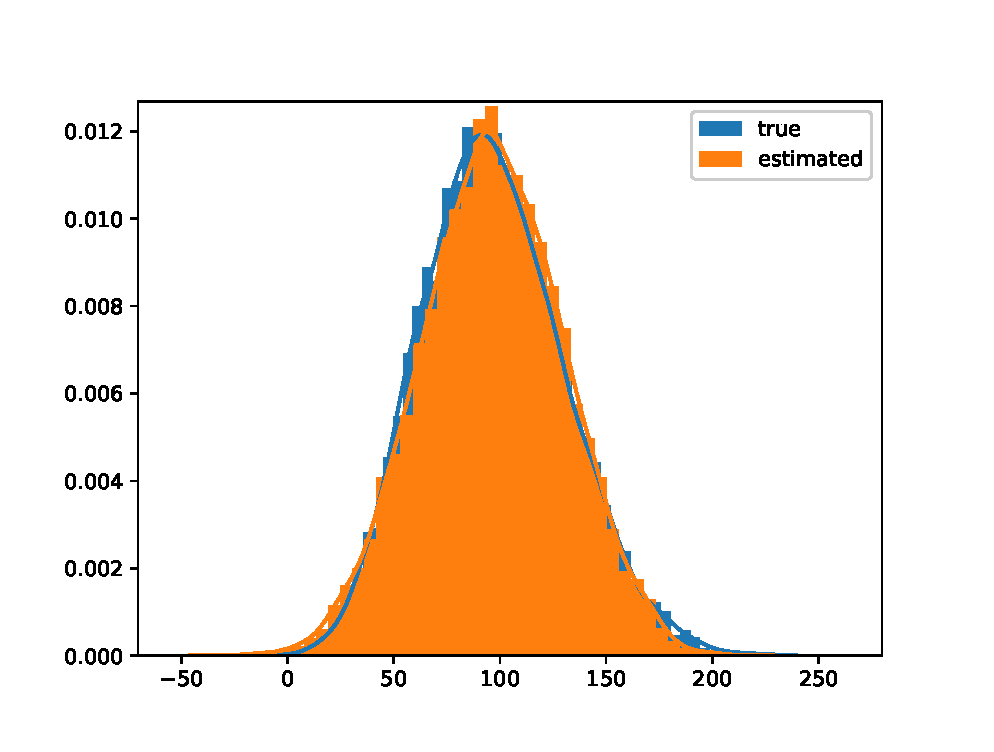
\includegraphics[width=\columnwidth]{d_testing}
\caption{Approximation of product of Gaussians.}
\label{fig:d_testing}
\end{figure}

\begin{figure}[t]
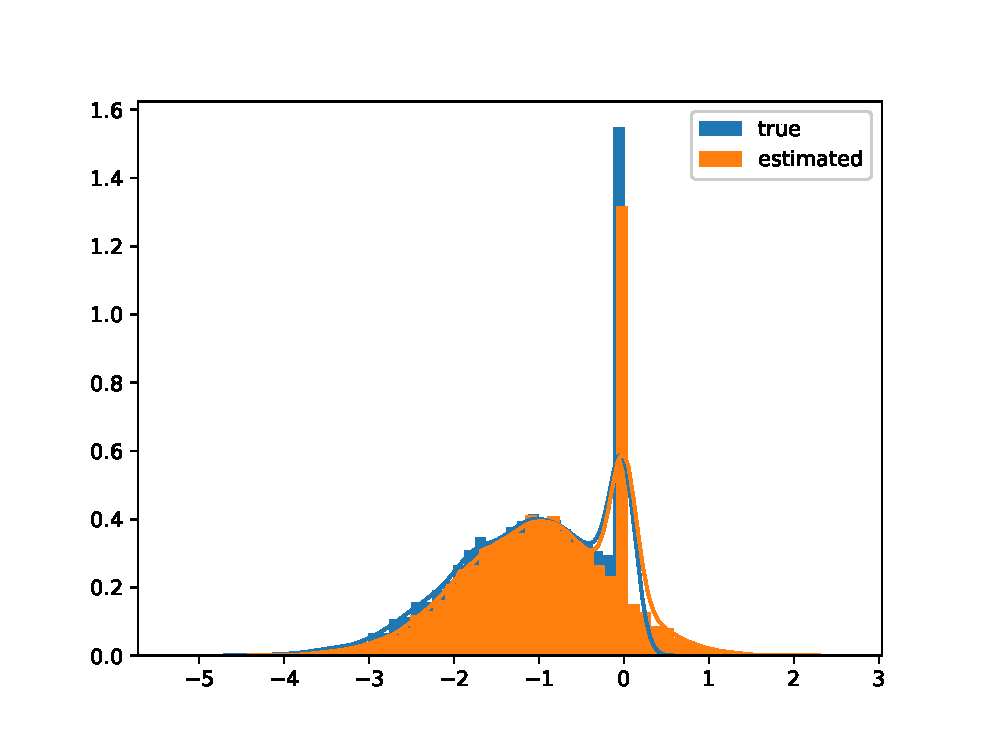
\includegraphics[width=\columnwidth]{z_new_testing}
\caption{Approximation of propagation through soft thresholding}
\label{fig:z_new_testing}
\end{figure}


\section{Backpropagation}
\label{sec:backpropagation}
\subsection{Likelihood}
We use the probabilistic backpropagation algorithm \citep{hernandez2015probabilistic} for computing parameters updates. It is based on assumed density filtering and expectation propagation and allows to update parameters of the distributions based on the derivative of the logarithm of the normalisation constant. 
The exact posterior \ref{eq:posterior} is approximated with a factorised distribution
\begin{align}
\begin{split}
q(\mathbf{W}, \mathbf{S}, \gamma, \eta) &= \prod_{d=1}^D\prod_{k=1}^K \mathcal{N}(w_{dk, l} | m^w_{dk, l}, v^w_{dk, l}) \\
&\times \prod_{d'=1}^D\prod_{d''=1}^D \mathcal{N}(s_{d'd'', l} | m^s_{d'd'', l}, v^s_{d'd'', l}) \\
&\times \text{Gam}(\gamma; \alpha^\gamma, \beta^\gamma) \text{Gam}(\eta; \alpha^\eta, \beta^\eta) 
\end{split}
\end{align}
The normalisation constant of the approximating distribution $q$ with the likelihood~\ref{eq:likelihood} term incorporated can be computed as follows
\begin{align}
\label{eq:Z}
\begin{split}
Z = \int \prod_{d=1}^{D} \big[&\mathcal{N}(\beta_d | f(\mathbf{y} ; \mathbf{S}, \mathbf{W}, \lambda), \gamma^{-1}) \\
 &q(\mathbf{S}, \mathbf{W}, \eta, \gamma)\big] \mathrm{d}\mathbf{S} \mathrm{d}\mathbf{W} \mathrm{d}\eta \mathrm{d}\gamma
 \end{split}
\end{align}
We sample $\mathbf{W}$, $\mathbf{S}$ from $q$ and get $\mathbf{z}_L$ - output from the network
\begin{align}
&Z \approx \int \prod_{d=1}^{D} \big[\mathcal{N}(\beta_d | [\mathbf{z}_L]_d, \gamma_d^{-1}) \nonumber \\
&\times (\omega^{z_L}_d \delta_0([\mathbf{z}_L]_d) + (1 - \omega^{z_L}_d)\mathcal{N}(m^{z_L}_d, v^{z_L}_d)) \nonumber\\
&\times \text{Gam} (\gamma_d; \alpha^\gamma, \beta^\gamma)\big]\mathrm{d}\mathbf{z}_L \mathrm{d}\boldsymbol\gamma  \nonumber\\
&= \prod_{d=1}^{D} \Big[\omega^{z_L}_d \int \big[\mathcal{N}(\beta_d | [\mathbf{z}_L]_d, \gamma_d^{-1})  \delta_0([z_L]_d) \nonumber \\
&\times \text{Gam} (\gamma_d; \alpha^\gamma, \beta^\gamma)\big]\mathrm{d}[{z}_L]_d \mathrm{d}\gamma_d  \nonumber\\
& + (1 - \omega^{z_L}_d)\int \big[\mathcal{N}(\beta_d | [\mathbf{z}_L]_d, \gamma_d^{-1})\mathcal{N}(m^{z_L}_d, v^{z_L}_d))  \nonumber\\
&\times \text{Gam} (\gamma_d; \alpha^\gamma, \beta^\gamma)\big]\mathrm{d}[{z}_L]_d \mathrm{d}\gamma_d\Big]  \nonumber\\
& = \prod_{d=1}^{D} \Big[\omega^{z_L}_d \int \mathcal{N}(\beta_d | 0, \gamma_d^{-1})  \text{Gam} (\gamma_d; \alpha^\gamma, \beta^\gamma) d\gamma_d  \nonumber\\
& + (1 - \omega^{z_L}_d)\int \big[\mathcal{T}(\beta_d | [\mathbf{z}_L]_d, \frac{\beta^\gamma}{\alpha^\gamma}, 2\alpha^\gamma)  \nonumber\\
&\times \mathcal{N}(m^{z_L}_d, v^{z_L}_d))\big] \mathrm{d}[{z}_L]_d\Big]  \nonumber\\
& \approx \prod_{d=1}^D \Big[\omega^{z_L}_d  \mathcal{T}(\beta_d | 0, \frac{\beta^\gamma}{\alpha^\gamma}, 2\alpha^\gamma) \nonumber \\ 
\label{eq:Z_approx}
&+ (1 - \omega^{z_L}_d)\mathcal{N}(m^{z_L}_d, \frac{\beta^\gamma}{\alpha^\gamma - 1} + v^{z_L})\Big]
\end{align}

The Student t density, can be parametrised in different ways. In this paper the following parametrisation is used 
\begin{equation}
\mathcal{T}(x; \mu, \beta, \nu) = \frac{\Gamma\left(\frac{\nu + 1}{2}\right)}{\Gamma\left(\frac{\nu}{2}\right)\sqrt{\pi \nu \beta}} \left(1 + \frac{(x - \mu)^2}{\nu\beta}\right)^{-\frac{\nu + 1}{2}}
\end{equation}
where $\Gamma(\cdot)$ denotes the Gamma function.

Then derivatives of $Z$ are computed w.r.t the weights and hyperparameters of the factorised distribution and then they are used for updates.
\subsection{Hyperparameter optimisation}
The only hyperparameter in the proposed Bayesian \textsc{lista} is the shrinkage parameter $\lambda$. It can be optimised using the Type II maximum likelihood procedure. The Type II likelihood, i.e. the evidence $p(\boldsymbol\beta | \mathbf{y}, \lambda)$, of the Bayesian \textsc{lista} is equal to the normalisation constant $Z$ (\ref{eq:Z}) computed for the whole training dataset $\boldsymbol\beta$. Given the approximation~(\ref{eq:Z_approx}) the optimal hyperparameter $\lambda$ can be found by a gradient-based optimiser.

\section{Experiments}

The following quality measures are used:
\begin{itemize}
\item $\text{\textsc{nmse}} (\text{normalised mean square error)})= \dfrac{\|\mathbf{X} - \widehat{\mathbf{X}}\|^2_{F}}{\|\mathbf{X}\|^2_{F}}$, where $\mathbf{X}$ is the true signal, $\widehat{\mathbf{X}}$ is the estimate, computed as the mean of the approximated posterior distribution, $\|\cdot\|_{F}$ is the Frobenius norm of a matrix;
\item $\text{F-measure} = 2\dfrac{\text{precision}\cdot\text{recall}}{\text{precision} + \text{recall}}$ between non-zero elements of the true signal $\mathbf{X}$ and non-zero elements of the estimate $\widehat{\mathbf{X}}$. 
\end{itemize}

We demonstrate the performance on small datasets to highlight that the proposed algorithm can learn when the dataset size is not sufficient for \textsc{lista}.

\subsection{Predictive performance on synthetic data}
First, the predictive performance of the proposed Bayesian \textsc{lista} is analysed on synthetic data. We generate $N_\text{train}=500$ sparse coefficients vectors $\boldsymbol\beta_n$ each of size $D = 100$. Coefficients $\boldsymbol\beta$ are generated from the spike-and-slab distribution with truncated slab: each component of $\beta_{nd}$ is zero with probability $0.8$ or is from standard Gaussian distribution without interval $(-0.1, 0.1)$ with probability $0.2$. Truncation of the zeros allows to remove from support pattern values with insignificant contributions \citep{xin2016maximal}. To simulate sparse observations, we have generated the random Gaussian design matrix $\mathbf{X} \in \mathbb{R}^{K \times D}$.  The observations are generated according to the \ref{eq:regression_problem} with zero-mean Gaussian noise with standard deviation $0.5$. 

We compare the proposed Bayesian \textsc{lista} with original \textsc{lista} algorithm \citep{gregor2010learning} and two deterministic algorithms: \textsc{ista} and Fast \textsc{ista} (\textsc{fista}) \citep{beck2009fast}. \textsc{fista} adds the momentum to \textsc{ista} and improves its convergence speed. We limit the number of iterations in these algorithms with $L$ that is the same as the number of layers in Bayesian \textsc{lista} and \textsc{lista}.

In the Figure \ref{fig:number_of_layers_synthetic} prediction performance for different number of layers $L$ is presented. The observation size is set as $K=50$. 

In the Figure \ref{fig:unsersampling_synthetic} prediction performance for different observation sizes $K$ is presented. The number of layers is set as $L=4$.

\begin{figure}[t]
\subfloat[\textsc{nmse} on train]{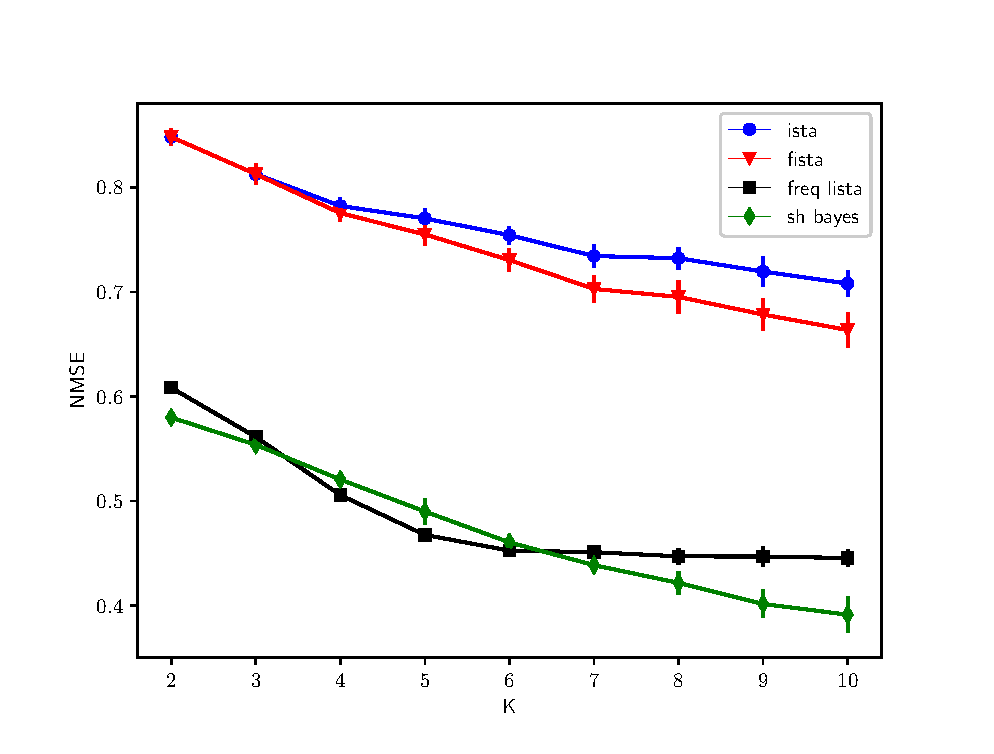
\includegraphics[width=0.5\columnwidth]{graphics/synthetic_number_of_layers/nmse_train}}
~
\subfloat[\textsc{nmse} on validation]{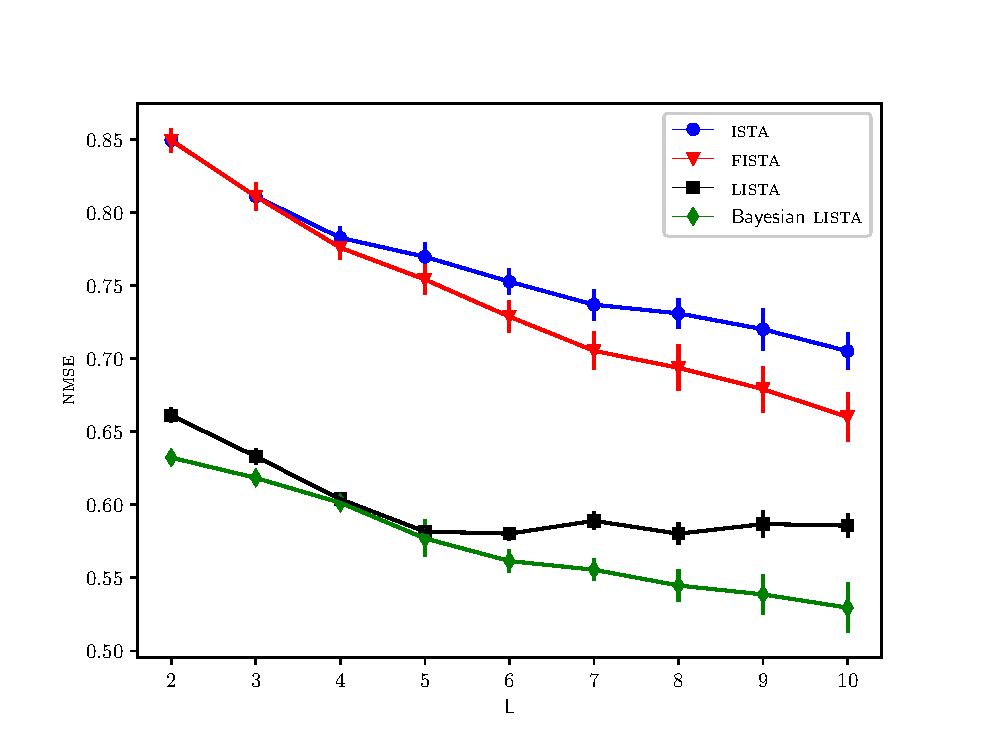
\includegraphics[width=0.5\columnwidth]{graphics/synthetic_number_of_layers/nmse_validation}}
\newline
\subfloat[F measure on train]{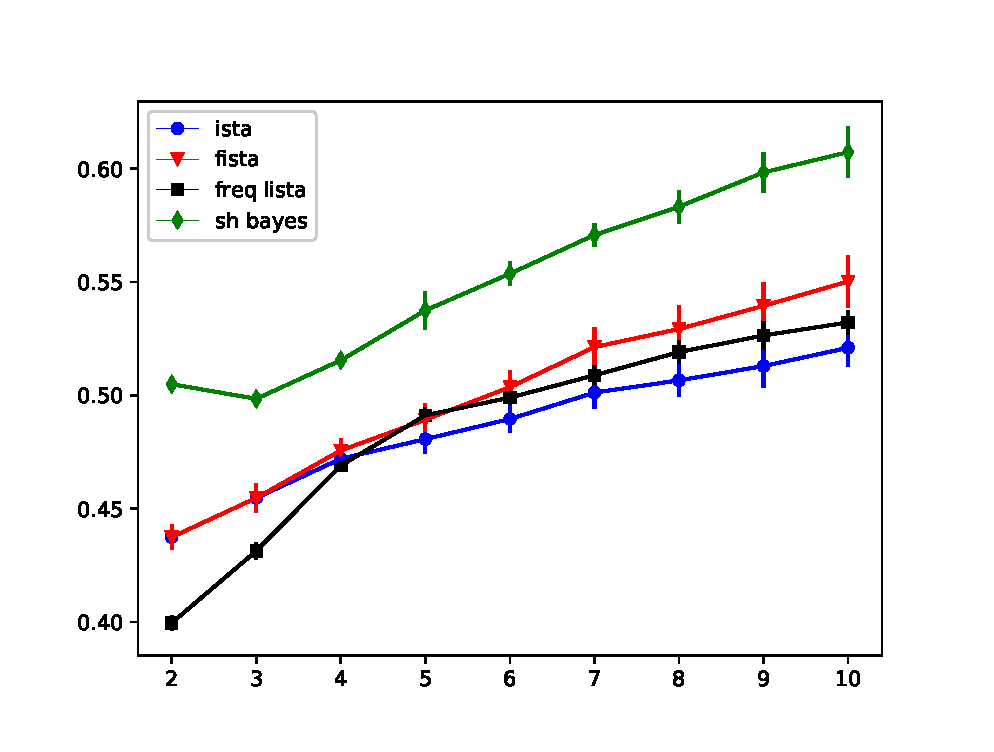
\includegraphics[width=0.5\columnwidth]{graphics/synthetic_number_of_layers/f_measure_train}}
~
\subfloat[F measure on validation]{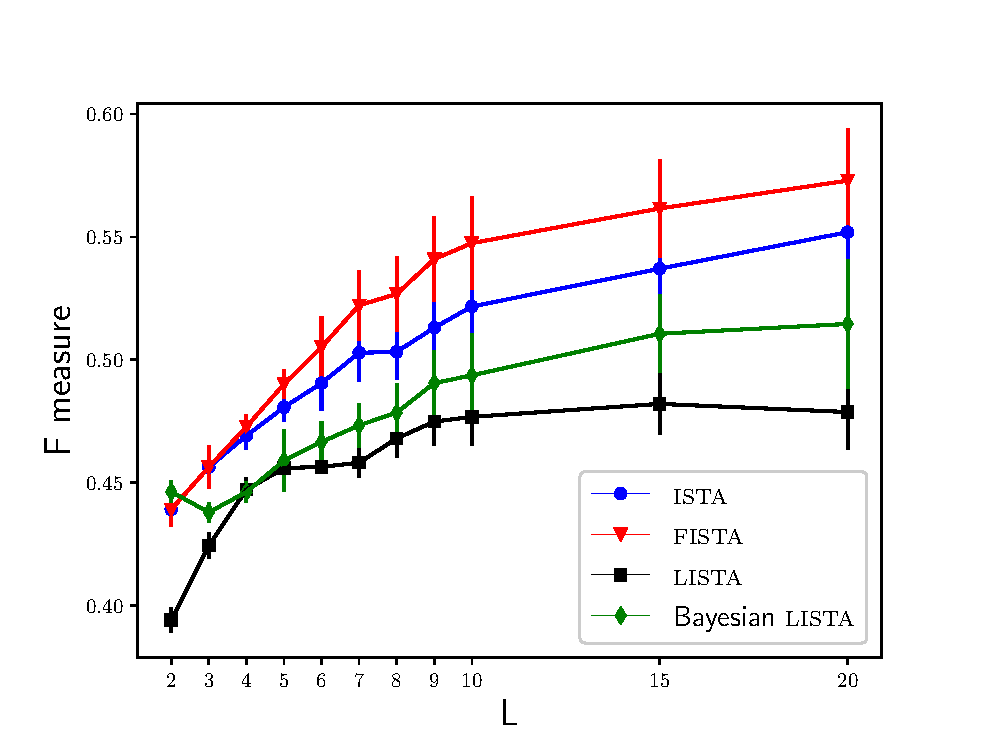
\includegraphics[width=0.5\columnwidth]{graphics/synthetic_number_of_layers/f_measure_validation}}
\caption{Number of layers on synthetic data}
\label{fig:number_of_layers_synthetic}
\end{figure}

\begin{figure}[t]
\subfloat[\textsc{nmse} on train]{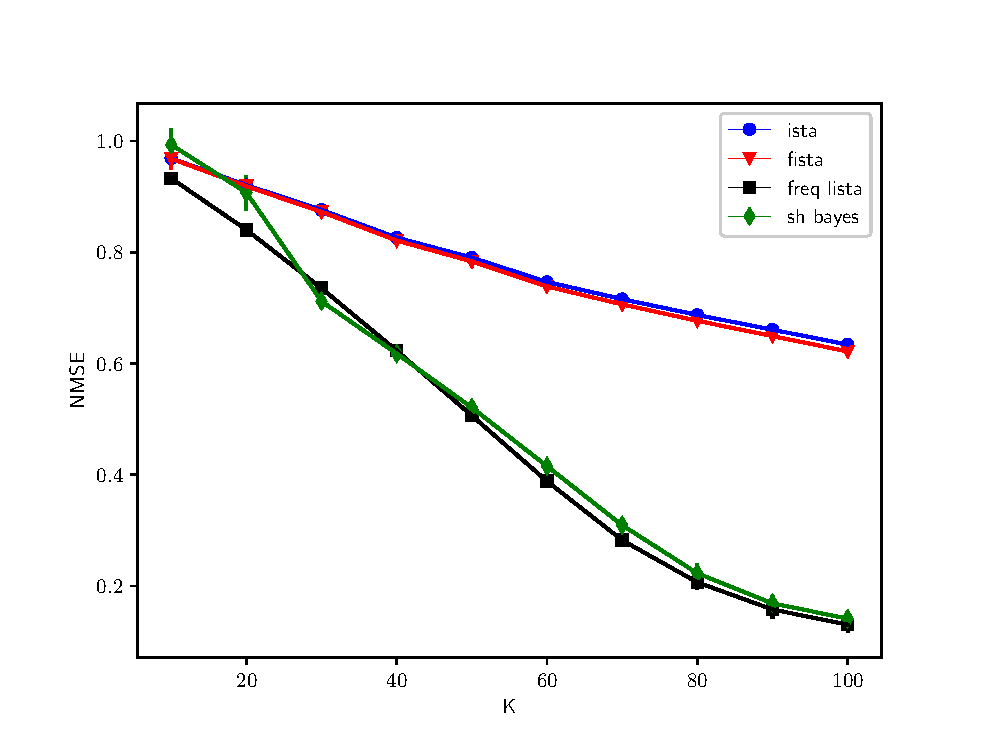
\includegraphics[width=0.5\columnwidth]{graphics/synthetic_undersampling/nmse_train}}
~
\subfloat[\textsc{nmse} on validation]{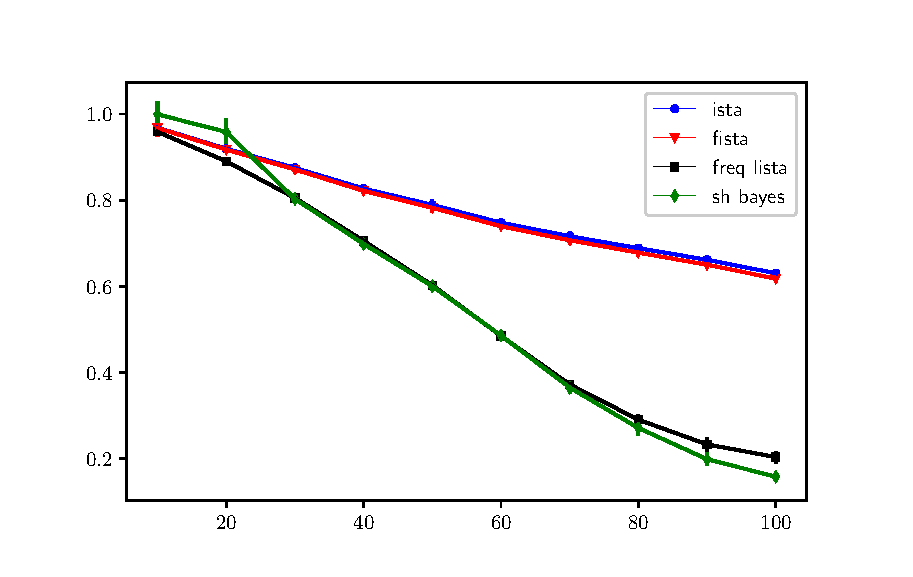
\includegraphics[width=0.5\columnwidth]{graphics/synthetic_undersampling/nmse_validation}}
\newline
\subfloat[F measure on train]{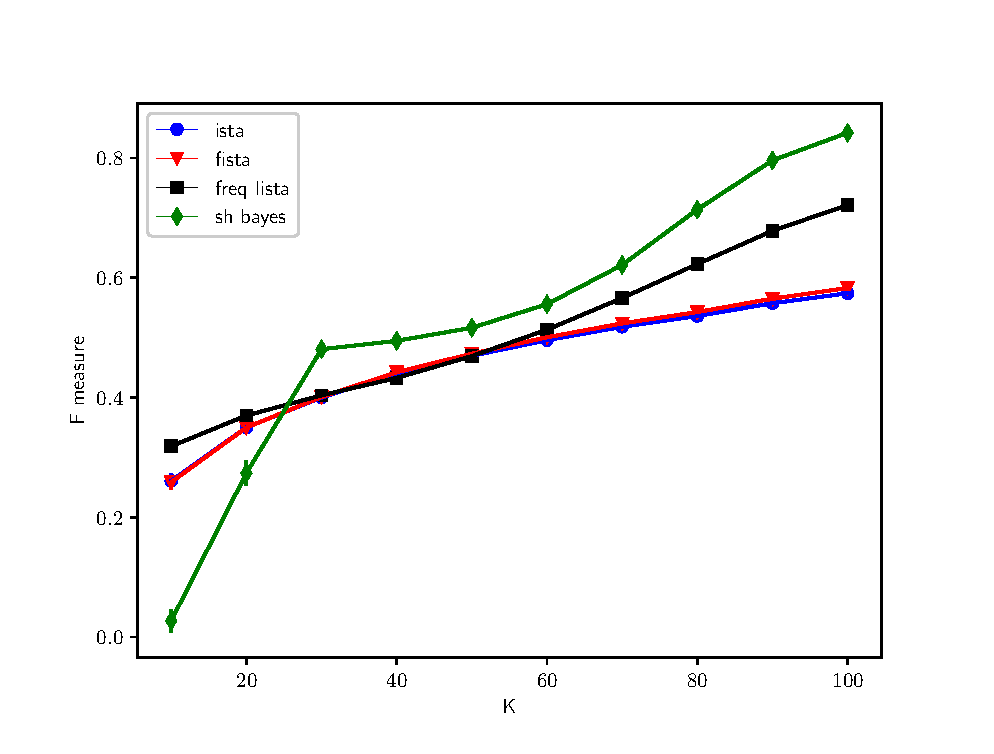
\includegraphics[width=0.5\columnwidth]{graphics/synthetic_undersampling/f_measure_train}}
~
\subfloat[F measure on validation]{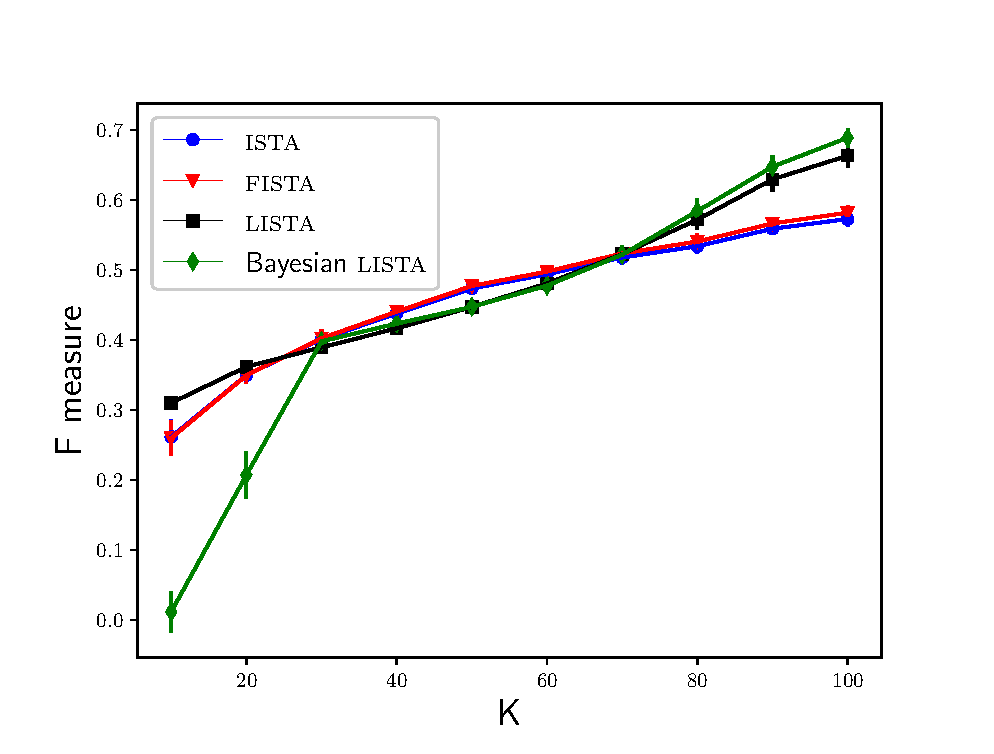
\includegraphics[width=0.5\columnwidth]{graphics/synthetic_undersampling/f_measure_validation}}
\caption{Size of observations on synthetic data}
\label{fig:unsersampling_synthetic}
\end{figure}

%We compare two versions of the proposed Bayesian LISTA: with shared weight matrices and with individual matrices at each layer --- and LISTA.

%The NMSE is presented in figure \ref{fig:validation_synthetic}.
%\begin{figure}[t]
%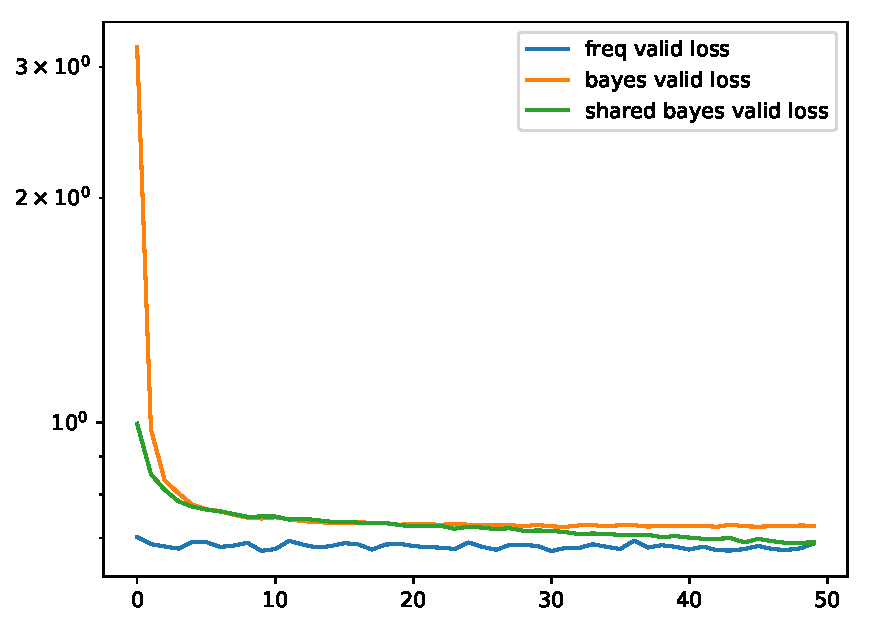
\includegraphics[width=\columnwidth]{loss_synthetic}
%\caption{Validation NMSE on synthetic data}
%\label{fig:validation_synthetic}
%\end{figure}

\subsection{MNIST}
Here we evaluate the proposed Bayesian \textsc{lista} in terms of predictive performance on the \textsc{mnist} dataset \citep{lecun2010mnist}. The dataset contains images of handwritten digits of size $28 \times 28 = 784$. The design matrix $\mathbf{X}$ is learned on 5000 images with the minibatch online algorithm \citep{mairal2009online}. The resulting size of $\mathbf{X}$ is $100 \times 784$. Then we generate observations as $\mathbf{y} = \mathbf{X}\boldsymbol\beta$, where $\boldsymbol\beta$ are images converted to vectors. We use randomly selected 1000 images for training and 100 for validation. 

Figure \ref{fig:validation} presents \textsc{nmse} loss on the validation set. 

Proposed Bayesian \textsc{lista} networks estimate posterior distribution for $\boldsymbol\beta$. Figure \ref{fig:posterior_samples} shows samples from the posterior for one of the validation data points and figure \ref{fig:posterior_distribution} shows the parameters of this posterior.
\begin{figure}[t]
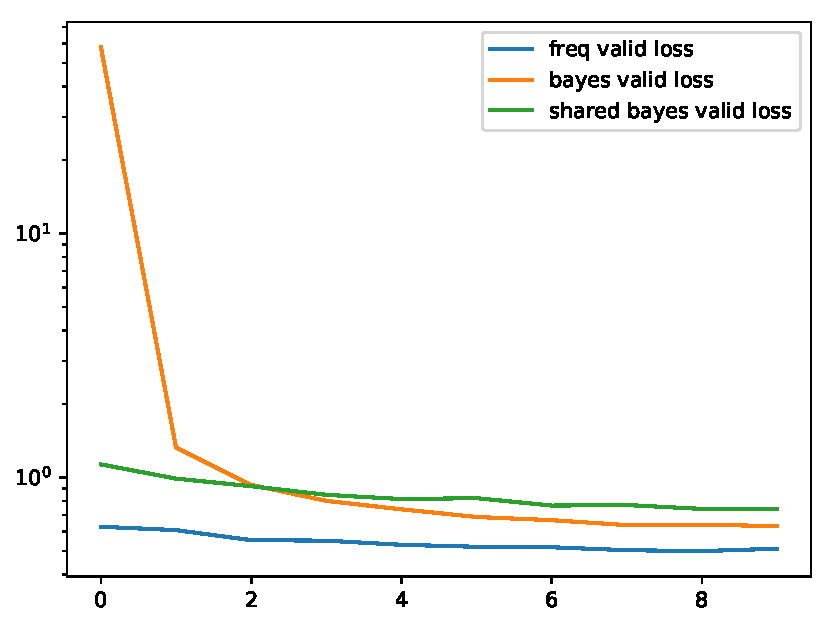
\includegraphics[width=\columnwidth]{loss}
\caption{Validation \textsc{nmse}}
\label{fig:validation}
\end{figure}
\begin{figure*}[t]
\subfloat[$\beta$ posterior mean]{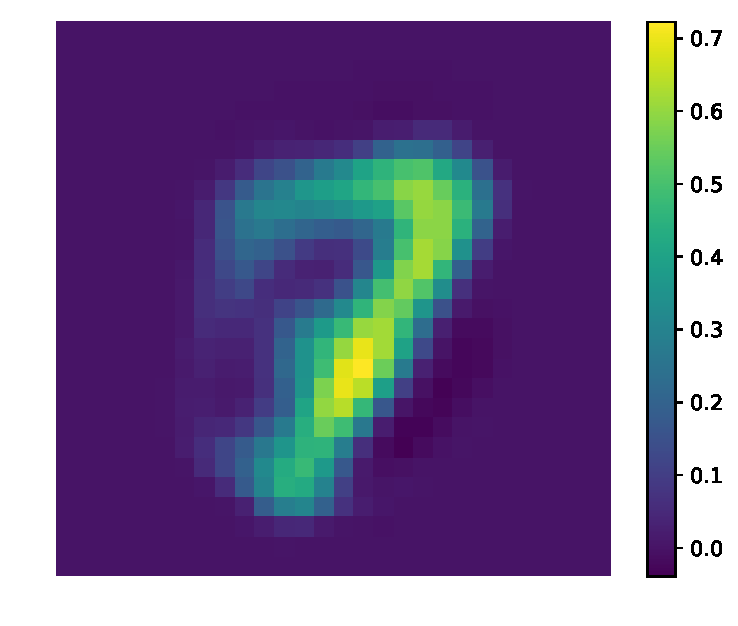
\includegraphics[width=0.66\columnwidth]{posterior_mean}}
\subfloat[$\beta$ posterior std]{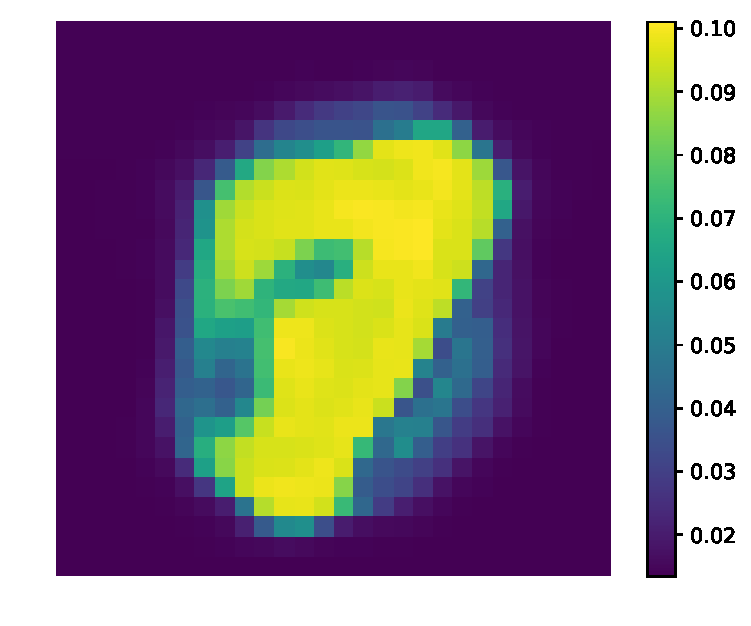
\includegraphics[width=0.66\columnwidth]{posterior_std}}
\subfloat[$\beta$ posterior spike indicator]{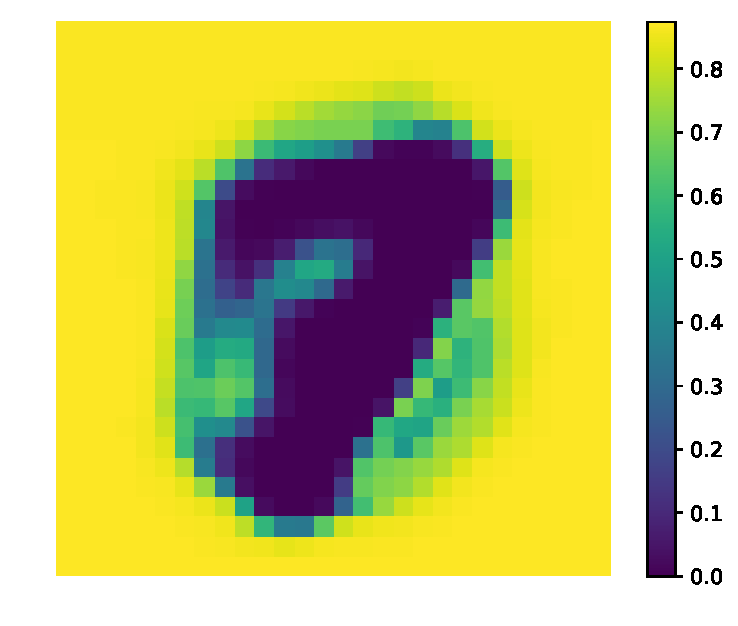
\includegraphics[width=0.66\columnwidth]{posterior_spike_indicator}}
\caption{Posterior for the digit 7.}
\label{fig:posterior_distribution}
\end{figure*}
\begin{figure*}[t]
\subfloat[]{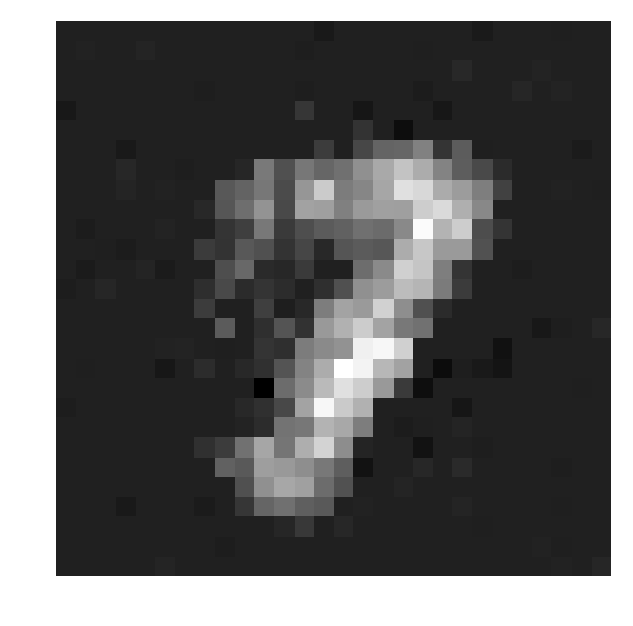
\includegraphics[width=0.66\columnwidth]{posterior_sample_0}}
\subfloat[]{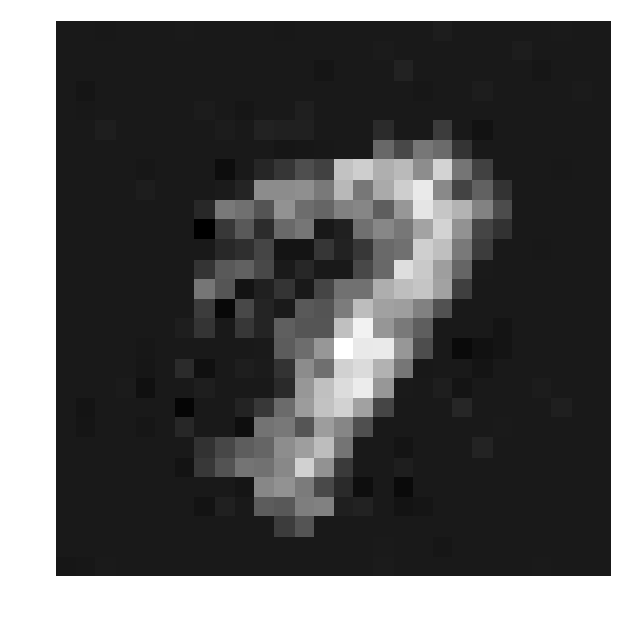
\includegraphics[width=0.66\columnwidth]{posterior_sample_1}}
\subfloat[]{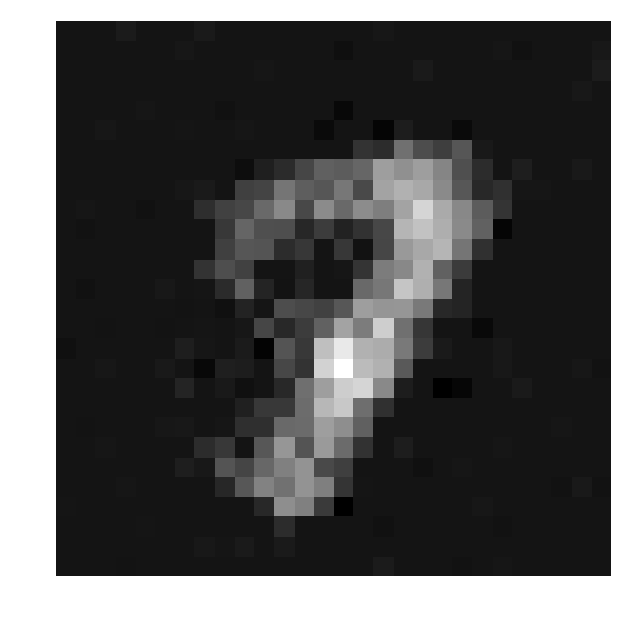
\includegraphics[width=0.66\columnwidth]{posterior_sample_2}}
\caption{Samples from the posterior for the digit 7.}
\label{fig:posterior_samples}
\end{figure*}

\section{Discussion}
As far as we are aware, this is the first implementation of Bayesian deep sparse coding algorithm, there are works on Bayesian sparsity in context of neural networks \citep{he2017bayesian}, but it is not the Bayesian Neural Network. We find not only correct predictions but also useful posterior estimates for the predictions that show how the model is confident in its decision. 
Though EP is not suited for distributed inference, some variations of ADF can be used \citep{li2015stochastic}. This allows the proposed approach to scale.

\bibliographystyle{agsm}
\bibliography{bibliography}

\end{document}
